\documentclass[10pt,aspectratio=169]{beamer}

\usetheme[progressbar=frametitle]{metropolis}
\usepackage{appendixnumberbeamer}

\usepackage{booktabs}
\usepackage[scale=2]{ccicons}

\usepackage{pgfplots}
\usepgfplotslibrary{dateplot}

\usepackage{xspace}
\newcommand{\themename}{\textbf{\textsc{metropolis}}\xspace}

\title{Buehler Committee Meeting}
\subtitle{2022}
% \date{\today}W
\date{}
\author{Matthew D. Buehler}
\institute{Department of Biological Sciences}
% \titlegraphic{\hfill\includegraphics[height=1.5cm]{logo.pdf}}
\begin{document}

\maketitle

\begin{frame}{Table of Contents}
  \setbeamertemplate{section in toc}[sections numbered]
  \tableofcontents%[hideallsubsections]
\end{frame}

\section[Personal Update]{Personal Update}

\begin{frame}{Spring and Summer 2022}  
\begin{itemize}
  \item Classes
    \begin{itemize}
      \item Evolutionary Biology
    \end{itemize}
  \item GTA Support
    \begin{itemize}
    \item Instructor of Record for Herpetology
    \end{itemize}
  \item Lab Work
    \begin{itemize}
      \item Created RAD libraries for \textit{Drymarchon}, \textit{Laticauda}, and \textit{Pachydactylus}
    \end{itemize}
\end{itemize}
\end{frame}

\begin{frame}{Fall 2021}
  \begin{itemize}
    \item GTA Support
    \begin{itemize}
      \item Teaching A\&P I and II 
    \end{itemize}
    \item Classes
    \begin{itemize}
      \item Pedigree Reconstruction
    \end{itemize}
    \item Lab Work
    \begin{itemize}
      \item Processing RAD data
    \end{itemize}
    \item Grants
    \begin{itemize}
      \item Submitted a proposal for Year 2 Funding of Section 6 Grant
    \end{itemize}
    
  \end{itemize}
\end{frame}

\section[Dissertation Status]{Dissertation Update}

\begin{frame}[fragile]{Indigo Snake Sequencing Efforts}
\begin{itemize}
  \item Approx. 300 individuals concentrated and ready for library prep
  \begin{itemize}
    \item About 50 breeders from the OCIC
    \item About 250 Wild Individuals
  \end{itemize}
  \item Additional 400 individuals available for future sequencing
  \item Whole Genome Sequence using PacBio Sequel II Platform
\end{itemize}
\end{frame}

\begin{frame}{Chapter 1: RADcap Panel Creation}
  \begin{itemize}
      \item Technical Chapter
      \item \textbf{Purpose:} Develop a panel of SNP loci from the 3RAD data that can be used to amplify informative loci for pedigree reconstruction and phylogenetic estimation. I will then develop a protocol that can be generalized and implemented for conservation of other squamate species. 

      \item \textbf{Goals:}
      \begin{itemize}
        \item Create a pipeline for mining informative SNP loci from 3RAD data
        \item Create a protocol for designing and testing MyBaits probes sets 
        \item Create a protocol for preparing RADcap libraries and sequencing 
        \item Create a pipeline for assembling the data, assessing data quality, and running preliminary analyses
        \item Create a script for reconstructing a pedigree for the OCIC breeding colony
      \end{itemize}
  \end{itemize}
\end{frame}

\begin{frame}{Chapter 2: Indigo Snake Phylogeography}
  % \begin{columns}[t]{}
    % \begin{column}[T]{5cm}
      \begin{itemize}
        \item \textbf{Biological Question} What abiotic factors contributed to the patterns of diversity seen in the EIS across Florida and southern Georgia?
        \begin{itemize}
        
        \item \textbf{Hypothesis 1} The Suwanee Strait led to genetic differentiation between northern and southern populations of \textit{Drymarchon couperi}
        \item \textbf{Hypothesis 2} Founder events after glacial retreat lead to the     establishment of genetically unique populations in southern Georgia. 
        \item \textbf{Hypothesis 3} The central ridge of Florida does act a barrier to gene flow between Atlantic and Gulf populations. Perhaps because the snakes typically forge and mate in the low lands they aren't crossing the ridge during meaningful times during the year
        \item \textbf{Hypothesis 4} The species originates in the north and founder events are actually down into Florida. Localized adaptation to warmer climates has lead to genetic differentiation between populations. 
      \end{itemize}
    \end{itemize}  
      %   \end{column}
  %   \begin{column}[T]{10cm}
  %     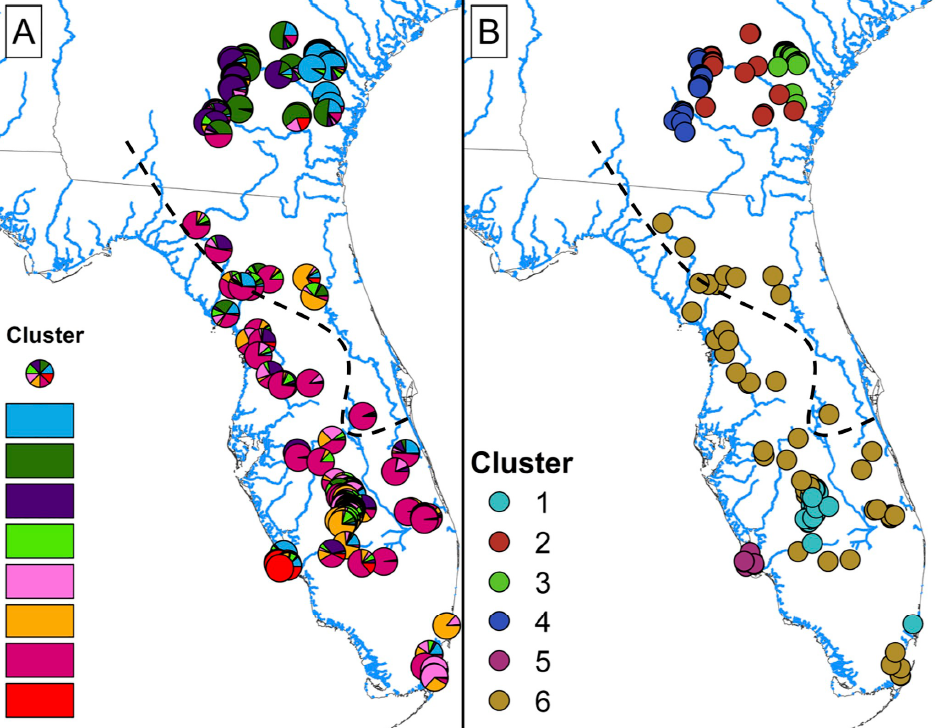
\includegraphics[height = 5.7cm]{media/indigo-snakes-genetic-clusters.PNG}
  %   \end{column}
  % \end{columns}
\end{frame}

\begin{frame}{Chapter 3: Indigo Snake Population Genetics}
      \begin{itemize}
       \item \textbf{Biological Question:} How connected are populations of \textit{D. couperi}?
        \begin{itemize}
          \item \textbf{Hypothesis 1:} Populations of southern Florida are actively sharing genes
          \item \textbf{Hypothesis 2:} Populations are restricted due to fragmented habitat and urbanization of the landscape. There is little to no gene flow between populations 
        \end{itemize}
      \end{itemize}  
\end{frame}

\begin{frame}{Chapter 4: SLiM Model for Population Viability}
\begin{itemize}
  \item \textbf{Biological Question:} How does the demographic and genetic make up of the OCIC breeding colony impact the chances of long term success of reintroduced populations?
  \begin{itemize}
    
    \item \textbf{Hypothesis 1:} Low genetic diversity in the OCIC breeding colony will lead to an increased frequency of the re-introduced population going extinct
    \item \textbf{Hypothesis 2:} Small effective population sizes will lead to rapid extinction of re-introduced indigo snake populations
    \item \textbf{Hypothesis 3:} Non-adaptive variation will result in strong directional selection in the re-introduced population leading to a drop in effective population size.
  \end{itemize}
  \item \textbf{Methods:}
    \begin{itemize}
      \item SLiM model developed in class last fall
      \item Based on the Folt et al. 2019 conservation model
      \item This model included many life history traits, but did not explicitly model how genetic diversity may shape outcomes
    \end{itemize}
  \end{itemize}
\end{frame}

\section[Year Goals]{Future Directions}

\begin{frame}{Spring and Summer 2023}
  \begin{itemize}
    \item GTA support
    \begin{itemize}
      \item 
    \end{itemize}
    \item Personal Goals
    \begin{itemize}
      \item Complete proposal by Spring Break
      \begin{itemize}
        \item Primarily pull from written grants
      \end{itemize}
      \item Do written exam by the end of the Spring semester
      \item Proposal seminar during the summer
      \begin{itemize}
        \item Be able to incorporate preliminary data
      \end{itemize}
    \end{itemize}
    \item Classes
    \begin{itemize}
      \item No
    \end{itemize}
  \end{itemize}

\end{frame}

\begin{frame}{Questions?}
  \begin{center}
    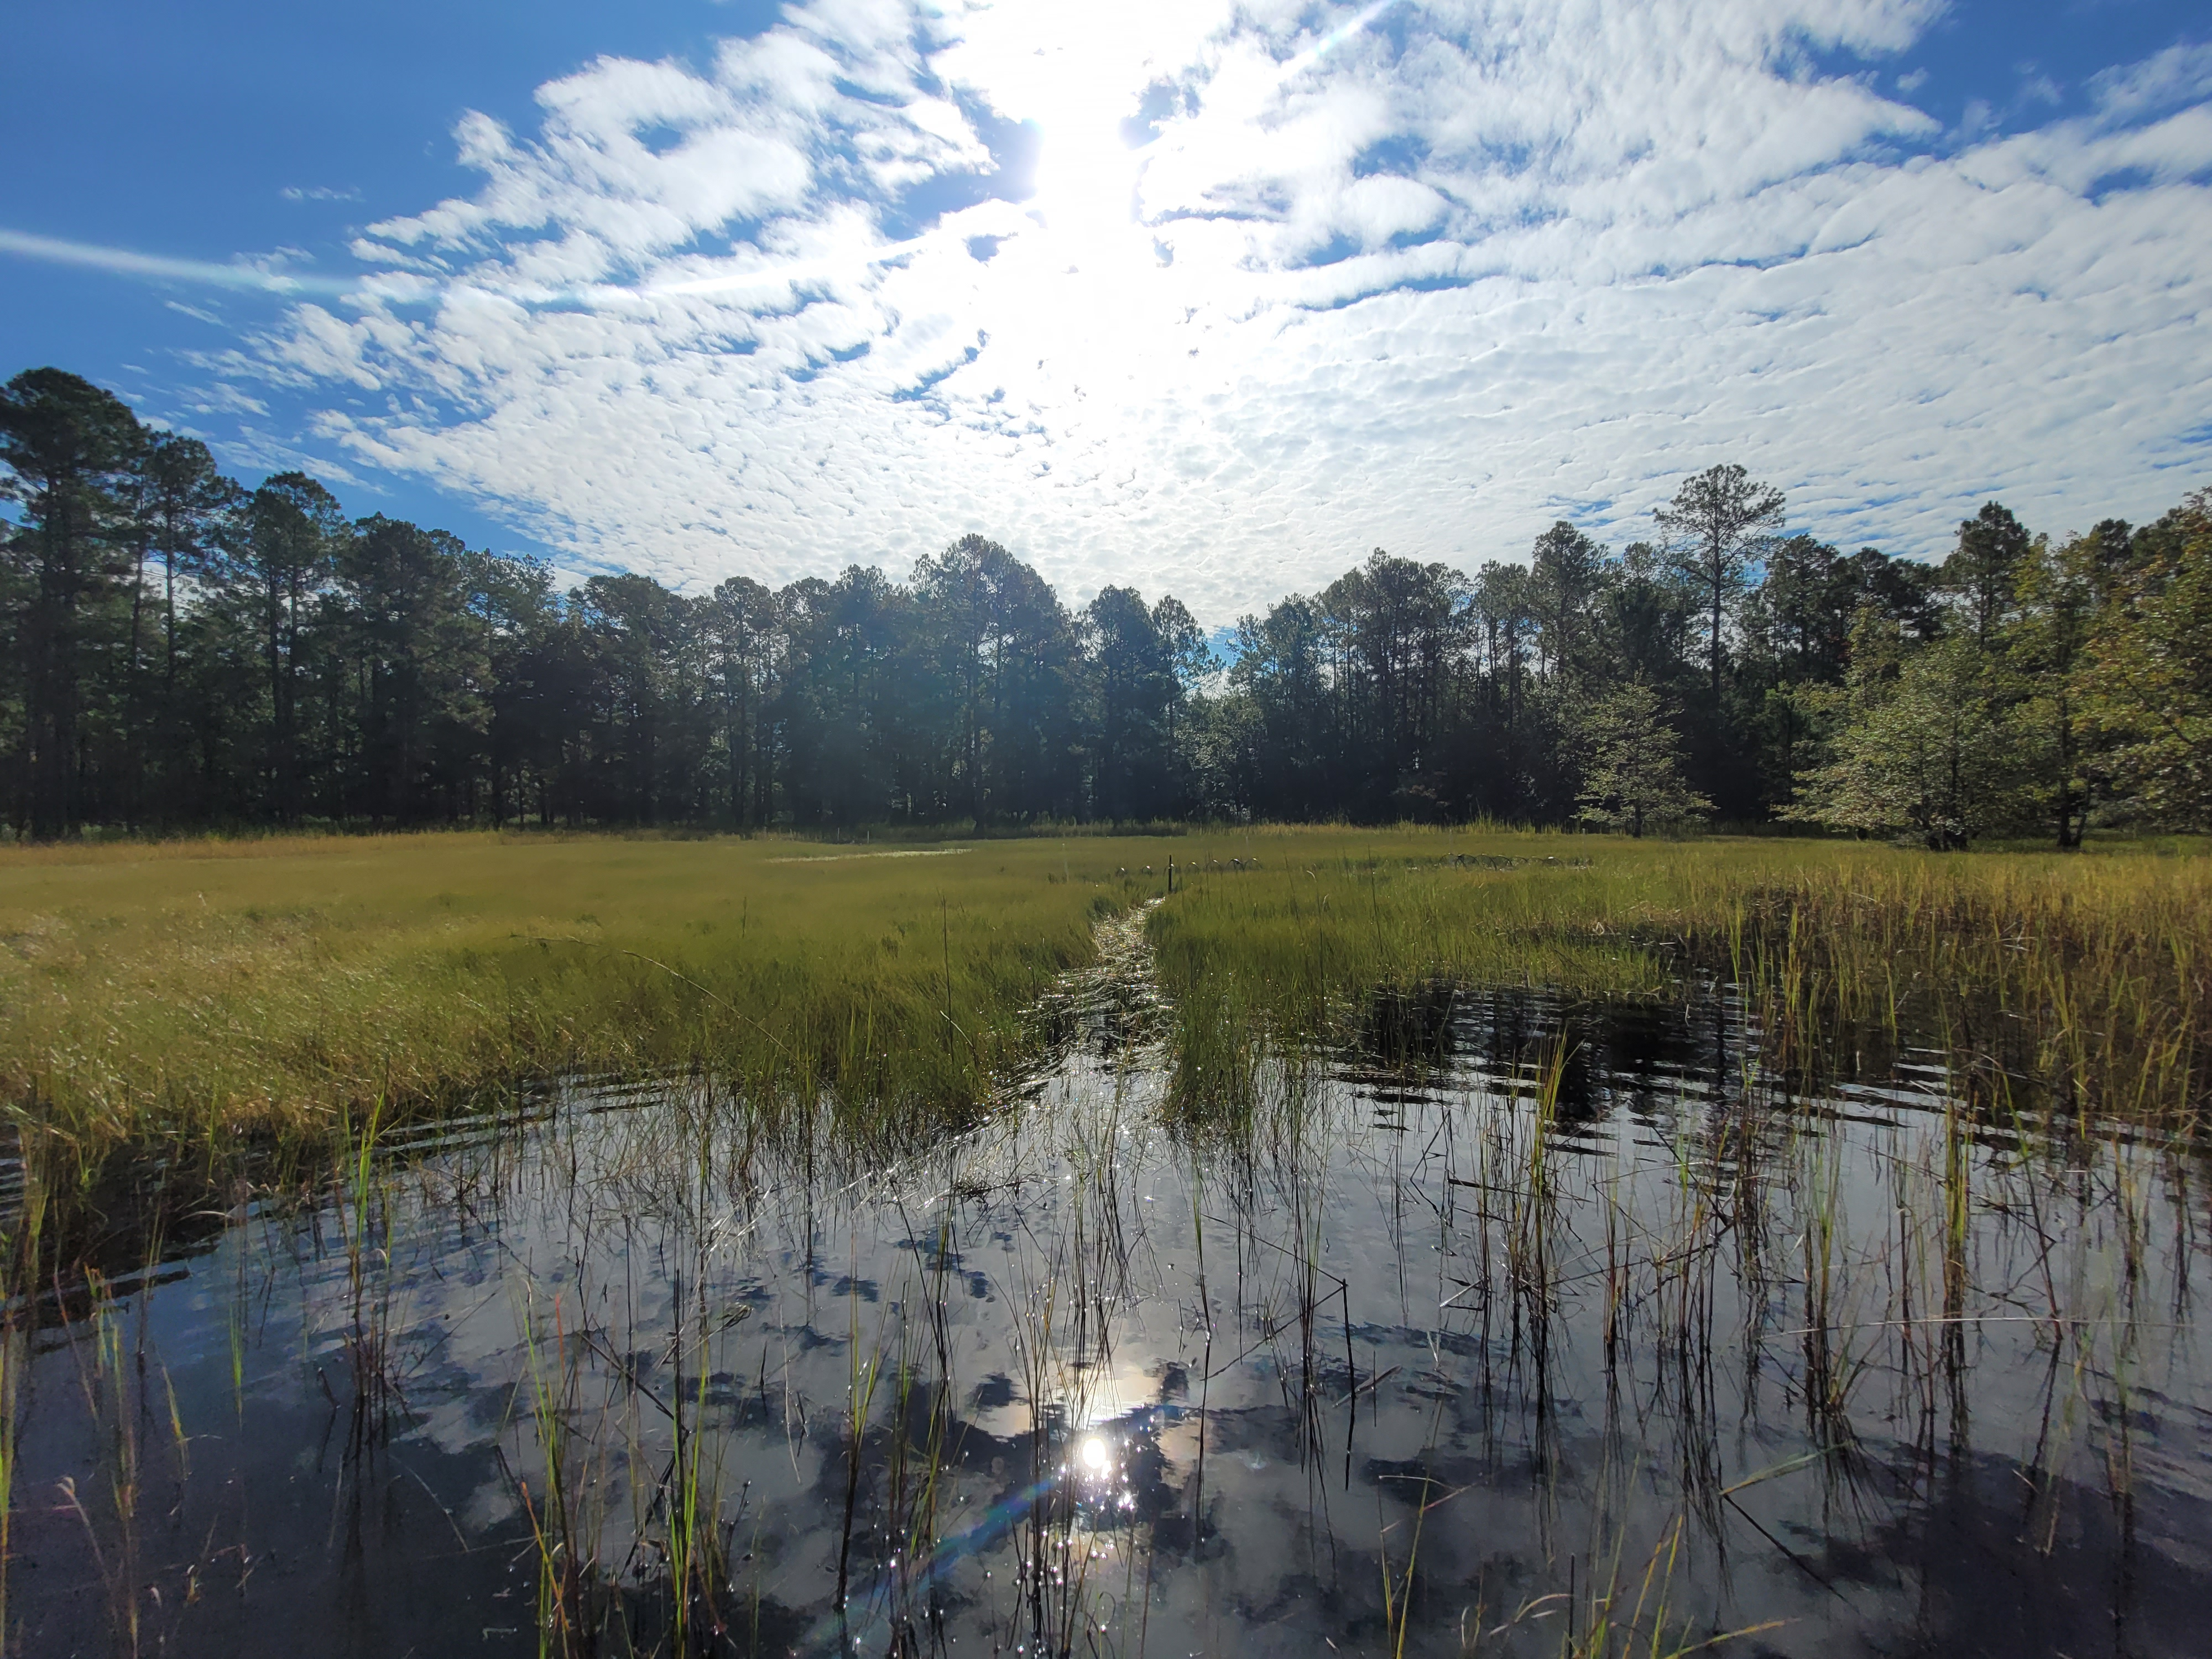
\includegraphics[height = 7.5cm]{media/conecuh-pond.jpg}    
  \end{center}

\end{frame}



\end{document}
